\documentclass[11pt]{beamer}
\usetheme{Warsaw}
\usepackage[utf8]{inputenc}
%\usepackage[magyar]{babel}
\usepackage[T1]{fontenc}
\usepackage{amsmath}
\usepackage{amsfonts}
\usepackage{amssymb}
\usepackage{graphicx}
\usepackage{xurl}
\usepackage{multimedia}
\usepackage{xurl}
\newenvironment{trienv}{\only{\setbeamertemplate{items}[triangle]}}{}
\newenvironment{squareenv}{\only{\setbeamertemplate{items}[square]}}{}
\author{Bendegúz Borkovits T7UR9P}
\title{Simulating detectors with Geant4 final presentation}
%\setbeamercovered{transparent} 
\setbeamertemplate{navigation symbols}{\insertframenumber/\inserttotalframenumber} 
%\logo{} 
\institute{Scientific Modelling Computer Laboratory} 
\date{May 2022} 
%\subject{} 
\begin{document}


\begin{frame}
\titlepage
\end{frame}

\begin{frame}{Geant4}
    \centering
    
\includegraphics[scale = 1.5]{g4logo.png}
    \begin{itemize}
        \vspace{0.7 cm}
        \item<tri@1-> Particle and Nuclear physics simulations.
        \vspace{0.2 cm}
        \item<tri@1-> Virtual detectors.
        \vspace{0.2 cm}
        \item<tri@1-> Visualization of events.
        \vspace{0.2 cm}
        \item<tri@1-> Support for: QT5, Python, multi-threading...
        \vspace{0.2 cm}
        \item<tri@1-> CMake project.
    \end{itemize}
\end{frame}

\begin{frame}{Progress in the first half of the semester}
    \begin{itemize}
        \item<tri@1-> Setting up the environment. (VirtualBox + Ubuntu 18.04)
        \vspace{0.2 cm}
        \item<tri@1-> Installing the software. (Geant4-10.7.03)
        \vspace{0.2 cm}
        \item<tri@1-> Testing it by running an example. (B1)
        \vspace{0.2 cm}
        \item<tri@1-> Learning the stepping stones of a simulation: (via Tutorial)
        \vspace{0.1 cm}
        \begin{itemize}
            \item<square@1-> Run manager. (main function)
            \vspace{0.1 cm}
            \item<square@1-> Detector construction. (geometry, material properties)
            \vspace{0.1 cm}
            \item<square@1-> Action runner. (computation)
            \vspace{0.1 cm}
            \item<square@1-> Particle generator. (particle properties)
            \vspace{0.1 cm}
            \item<square@1-> Physics list. (laws of physics)
        \end{itemize}
        \vspace{0.2 cm}
        \item<tri@1-> Fixing issues. (optical photons, environment)
        \vspace{0.2 cm}
        \item<tri@1-> Showcasing some output and saving data.
    \end{itemize}
\end{frame}

\begin{frame}{Cherenkov radiation (a proton and optical photons)}
    \centering
    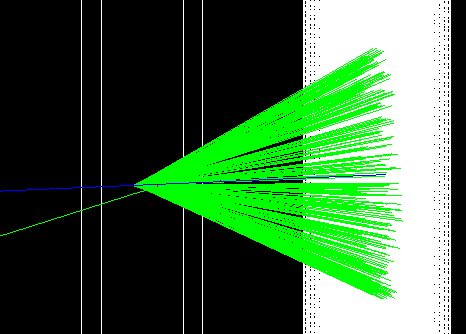
\includegraphics[scale = 0.7]{sensitive_detectors.png}
    \begin{itemize}
        \item<tri@1-> Propagating the photons through the detector.
        \item<tri@1-> Creating sensitive detectors.
        \item<tri@1-> Electromagnetic interaction enabled in physics list.
        \item<tri@1-> A proton passes through the detector and emits photons.
        \item<tri@1-> Beta-electrons can also appear.
        \item<tri@1-> Preparing output for analysis.
    \end{itemize}
\end{frame}

\begin{frame}{Preparing the yielded data for analysis}
    \begin{itemize}
        \item<tri@1-> Possibilities for saving data: ROOT, XML, CSV, HBOOK
        \item<tri@1-> Installed ROOT and checked the output. (g4root)
        \item<tri@1-> Opted for CSV for easier evaluation. (g4csv)
    \end{itemize}
\begin{columns}
\begin{column}{0.5\textwidth}
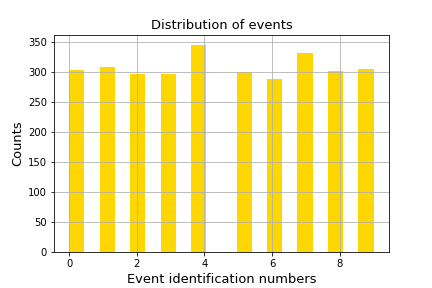
\includegraphics[scale = 0.4]{histo.png}
\begin{itemize}
    \item<tri@1-> Counts = Number of photons in an event.
    \item<tri@1-> Uniformly distributed: mean of $308\pm17$ photons.
\end{itemize}
\end{column}
\begin{column}{0.5\textwidth}
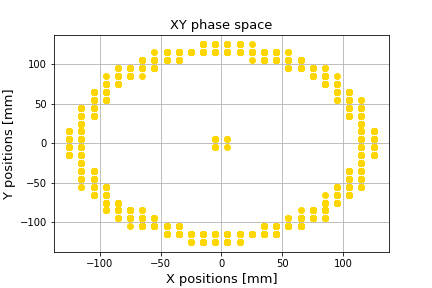
\includegraphics[scale = 0.4]{xy_phase.png}
\begin{itemize}
    \item<tri@1-> Footprint of the photon cone.
    \item<tri@1-> Low probability events in the middle.
    \end{itemize}
\end{column}
\end{columns}
\end{frame}

\begin{frame}{Progress in the second half of the semester}
    \begin{itemize}
        \item<tri@1-> Studying the structure of the NEBULA detector.
        \vspace{0.2 cm}
        \item<tri@1-> Trying to install smsimulator and failing at that.
        \vspace{0.2 cm}
        \item<tri@1-> Using the simulation made by Balázs Pál.
        \vspace{0.2 cm}
        \item<tri@1-> Making smaller modifications to the program and some fixing.
        \vspace{0.2 cm}
        \item<tri@1-> Projecting a neutron beam through the detector.
        \vspace{0.2 cm}
        \item<tri@1-> Exploring different physics lists.
        \vspace{0.2 cm}
        \item<tri@1-> Grouping the relative number of particles via:
        \begin{itemize}
        \vspace{0.1 cm}
            \item<square@1-> particle type,
            \vspace{0.1 cm}
            \item<square@1-> generating process type,
            \vspace{0.1 cm}
            \item<square@1-> detection volume type.
        \end{itemize}
        \vspace{0.2 cm}
        \item<tri@1-> Grouping the deposited energy by the same categories.
        \vspace{0.2 cm}
        \item<tri@1-> Doing some analysis with the neutron generated protons.
    \end{itemize}
\end{frame}

\begin{frame}{NEBULA detector}
    \begin{itemize}
        \item<tri@1-> Neutron (NEUT) and charged particle (VETO) detector modules.
        \vspace{0.2 cm}
        \item<tri@1-> Enough modules for only two walls.
        \vspace{0.2 cm}
        \item<tri@1-> Simulating only 20 NEUT modules here.
        \vspace{0.2 cm}
    \end{itemize}
    \centering
    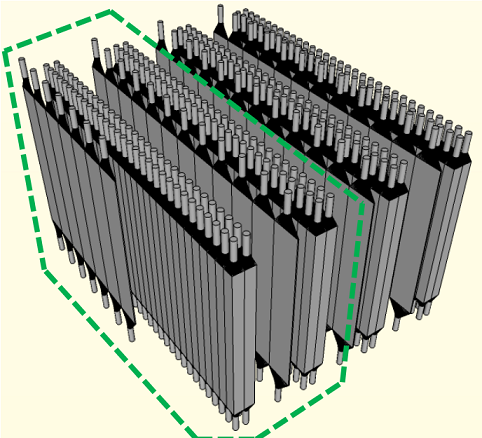
\includegraphics[scale = 0.6]{walls.png}
\end{frame}


\begin{frame}{Neutron beam}
        \begin{itemize}
        \item<tri@1-> 100 uniformly distributed neutrons, each has 100 MeV energy.
        \vspace{0.2 cm}
        \item<tri@1-> Many particles are difficult to visualize properly.
        \vspace{0.2 cm}
    \end{itemize}
    \centering
    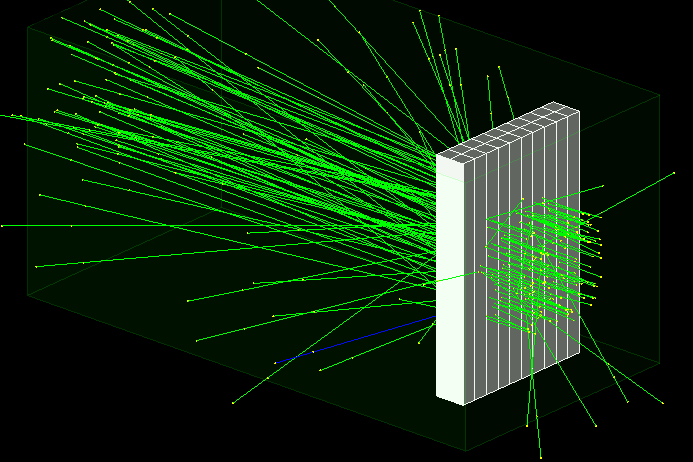
\includegraphics[scale = 0.68]{qbbc_neutbeam.png}
\end{frame}

\begin{frame}{Physics lists}
    \begin{itemize}
        \item<tri@1-> QBBC: Geant4 Bertini and Binary cascade models
        \vspace{0.2 cm}
        \item<tri@1-> QGSP: Quark Gluon String model for high energy hadronic interactions of protons, neutrons, pions, and Kaons
        \vspace{0.2 cm}
        \begin{itemize}
            \item<square@1-> QGSP\_BERT\_HP: Geant4 Bertini cascade, data driven high precision neutron package (HP)
            \vspace{0.2 cm}
            \item<square@1-> QGSP\_BIC\_HP: Geant4 Binary cascade, binary light ion cascade
            \vspace{0.2 cm}
            \item<square@1-> QGSP\_INCLXX: Liege Intranuclear Cascade model
            \vspace{0.2 cm}
            \item<square@1-> QGSP\_INCLXX\_HP: Improved version of the previous one
        \end{itemize}
    \end{itemize}
    
\begin{alertblock}{Difference in output}
In the end, the main difference lies with the different types of low energy by-product particles that the physics lists allow to surface.
\end{alertblock}
\end{frame}

\begin{frame}{Results of classification (relative number of particles)}
    \centering
    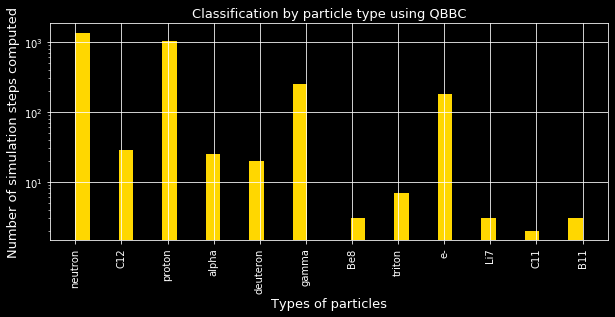
\includegraphics[scale = 0.46]{classpart.png}
    \begin{itemize}
    \vspace{0.2 cm}
        \item<tri@1-> Neutrons and protons dominate.
        \vspace{0.2 cm}
        \item<tri@1-> Hadronic processes dominate.
        \vspace{0.2 cm}
        \item<tri@1-> Fewer particles were detected on the sides of the wall.
        \vspace{0.2 cm}
        \item<tri@1-> Many by-products are present with lesser significance.
    \end{itemize}
\end{frame}

\begin{frame}{Results of classification (deposited energy)}
    \centering
    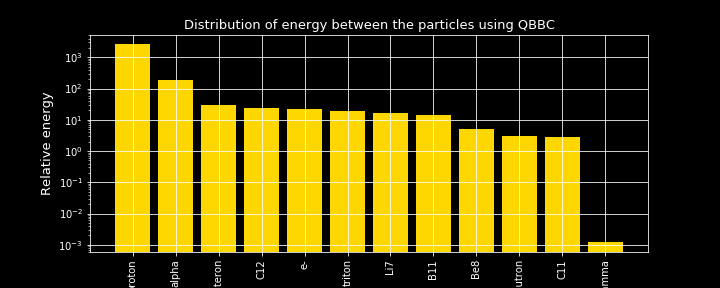
\includegraphics[scale = 0.46]{prenpart.png}
    \begin{itemize}
    \vspace{0.2 cm}
        \item<tri@1-> Protons deposited the largest amount of energy.
        \vspace{0.2 cm}
        \item<tri@1-> Hadronic processes generated the most energy.
        \vspace{0.2 cm}
        \item<tri@1-> Almost all of the energy was deposited into the NEUT modules. (Barely any into the enveloping volumes.)
    \end{itemize}
\end{frame}

\begin{frame}{Analysis with protons pt. 1}
    \begin{itemize}
        \item<tri@1-> Protons are the most prominent by-products in this process.
        \vspace{0.4 cm}
    \end{itemize}
    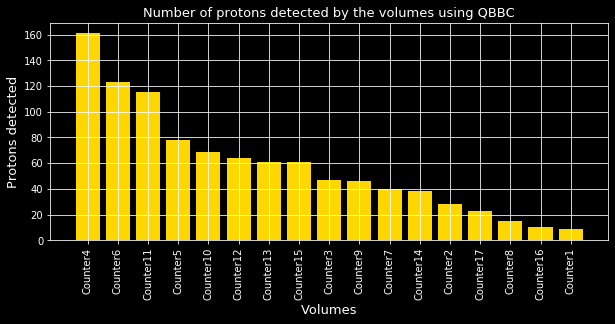
\includegraphics[scale = 0.5]{proton_num.png}
\end{frame}

\begin{frame}{Analysis with protons pt. 2}
    \begin{itemize}
        \item<tri@1-> It would be nice to measure the distribution of deposited energy by a proton in each NEUT modules.
        \vspace{0.2 cm}
        \item<tri@1-> Taking into account detector efficiency.
        \vspace{0.4 cm}
    \end{itemize}
    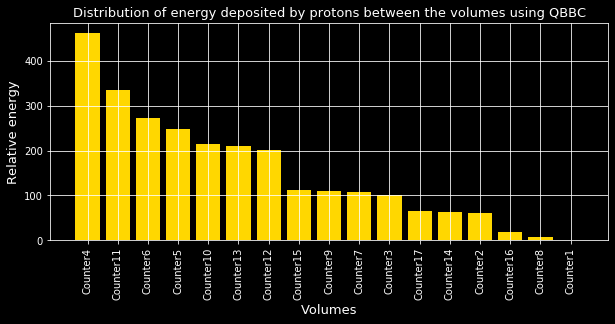
\includegraphics[scale = 0.5]{proton_en.png}
\end{frame}

\begin{frame}{Analysis with protons pt. 3}
    \begin{itemize}
        \item<tri@1-> Problem: Each detection of the same particle counts as a separate particle of the same type.
        \vspace{0.4 cm}
    \end{itemize}
    \centering
    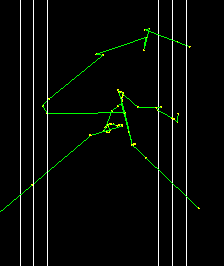
\includegraphics[scale = 1]{proton_bounce.png}
\end{frame}

\begin{frame}{Analysis with protons pt. 4}
    \begin{itemize}
        \item<tri@1-> Need to include TrackID to track individual particles.
        \item<tri@1-> Can also include EventID to track whole events.
        \item<tri@1-> TrackID by Volume matrix. (Total deposited energy.)
    \end{itemize}
    \centering
    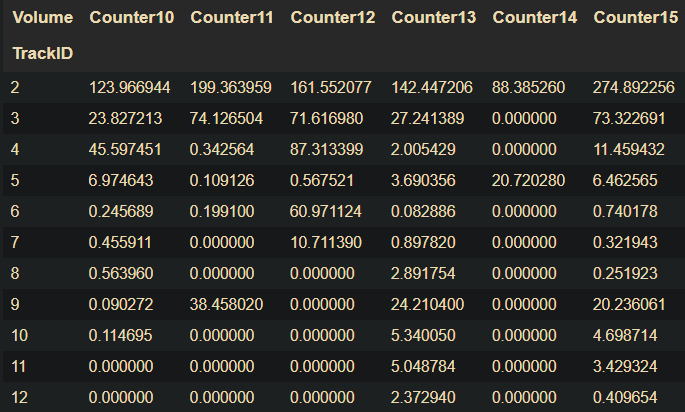
\includegraphics[scale = 0.7]{matrix.png}
\end{frame}

\begin{frame}{Analysis with protons pt. 5}
Results can be viewed here:
    \begin{itemize}
        \item<tri@1-> \url{https://github.com/borbende/Scientific-Modelling-Computer-lab/blob/main/the_end/figures/mat1.png}
        \item<tri@1-> \url{https://github.com/borbende/Scientific-Modelling-Computer-lab/blob/main/the_end/figures/mat2.png}
        \item<tri@1-> \url{https://github.com/borbende/Scientific-Modelling-Computer-lab/blob/main/the_end/figures/mat3.png}
        \item<tri@1-> \url{https://github.com/borbende/Scientific-Modelling-Computer-lab/blob/main/the_end/figures/mat4.png}
        \item<tri@1-> \url{https://github.com/borbende/Scientific-Modelling-Computer-lab/blob/main/the_end/figures/mat5.png}
    \end{itemize}
    
    \begin{block}{Differences between runs}
    Number of protons, energy deposited, accountable volumes.
    \end{block}
\end{frame}

\begin{frame}{Sources and tools}
    \begin{itemize}
        \item<tri@1-> Oracle VM VirtualBox: \url{https://www.virtualbox.org/wiki/Downloads}
        \item<tri@1-> Ubuntu 18.04: \url{https://ubuntu.com/download/desktop}
        \item<tri@1-> Geant4: \url{https://geant4.web.cern.ch/support/download}
        \item<tri@1-> ROOT: \url{https://root.cern/install/}
        \item<tri@1-> Python: \url{https://www.anaconda.com/}
        \item<tri@1-> Tutorials: \url{https://www.youtube.com/channel/UCyxwnZPodqQR0hUo5sapRFw}
        \item<tri@1-> NEBULA detector official site: \url{http://be.nucl.ap.titech.ac.jp/~nebula/index.php}
        \item<tri@1-> Smsimulator official site: \url{http://be.nucl.ap.titech.ac.jp/~nebula/simulator.php}
        \item<tri@1-> RI Beam factory informations: \url{https://www.riken.jp/en/collab/resources/ribf/}
        \item<tri@1-> Balázs Pál simulation: \url{https://github.com/masterdesky/ELTE_Modelling_Lab_2021/tree/main/project/project_nebula/NEBULA}
    \end{itemize}
\end{frame}

\begin{frame}{End notes}
\begin{itemize}
    \item<tri@1-> Geant4 is very hard to master.
    \vspace{0.1 cm}
    \item<tri@1-> Even with tutorials, coding and debugging can be a nightmare.
    \item<tri@1-> Significant progress was made in the project during the semester.
    \vspace{0.1 cm}
    \item<tri@1-> Not all aims were accomplished: automatization.
    \vspace{0.1 cm}
    \item<tri@1->Numerous issues arose: environmental, compatibility, coding issues which delayed progress sometimes by weeks.
    \vspace{0.1 cm}
    \item<tri@1-> All in all, I have acquired basic knowledge about working with Geant4 and analysing data yielded by its simulations.
    \vspace{0.1 cm}
    \item<tri@1-> My github: \url{https://github.com/borbende/Scientific-Modelling-Computer-lab}
    \vspace{0.1 cm}
    \item<tri@1-> Consultants provided invaluable help. Thank you, Ákos Horváth and Balázs Pál!
\end{itemize}

    \centering
    \alert{Thank you for your attention!}
    
\end{frame}




\end{document}
